\setModuleTitle{Introduction to Linux Operating System}
\setModuleAuthors{%
  Ramona Rogers, Research Services, University of Adelaide \mailto{ramona.rogers@adelaide.edu.au}\\
}
\setModuleContributions{%
  Exequiel Sepulveda, Research Services, University of Adelaide \mailto{exequiel.sepulvedaescobedo@adelaide.edu.au} \\
}

%----------------------------------------------------------------------------------------
% MODULE TITLE PAGE
%----------------------------------------------------------------------------------------
% BEGIN: Module Title Page
%  * The chapter page will always appear on odd numbered page
\chapter{\moduleTitle}

Linux has become the most used operating system for servers, and for High Performance Computing (HPC) in particular. That is the motivation to bring you this workshop.
The main goal is to show what a Linux OS is and how to use it, focus on Phoenix, the HPC facilities for supercomputing at The University of Adelaide.

\section{Components of the Linux Operating System}

An operating system is a dedicated computer program whose primary purpose is to execute other programs, to manage the hardware and system resources for those programs.
The operating system sits on top of the hardware and it is on what the general programs run.
\\
You probably are familiarised with Windows operating system, but there are many others, among the most popular are: Linux, macOS and Android.
\\
Phoenix uses Linux as operating system.
\\
The Linux operating system can be depicted as a series of layers as hardware, device-drivers, kernel, shells and special applications.

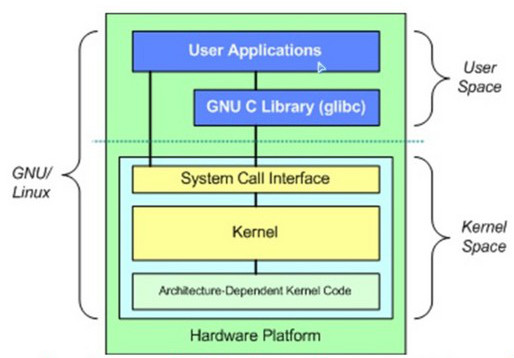
\includegraphics{linux_components}

\subsection{Hardware}
In our case the hardware are the parts of the computer like:
\begin{itemize}
\item Central processing unit or CPU. The CPU executes programs, which are located in the memory. Modern CPU has many cores enabling a first layer of parallelism.
\item Random access memory, in short RAM or memory. 
The memory allows fast access to the instructions and data that the CPU needs and because the RAM is limited it will store only information for immediate use.
Permanent data is kept in auxiliary storage on devices of the input/output subsystem.
\item Input/output subsystem contains devices called peripherals that provide input and output for the system as well as the user, and short-term and long-term storage for the processes and data. 
These devices include among others:
\begin{itemize}
\item Hard disk(s)
\item Various added cards (ie video, sound, USB-ports)
\item Monitor(s)
\item Keyboard and mouse
\item Network
\end{itemize}
\end{itemize}

On Phoenix the most relevant parts and devices are: Hard disks, RAM, Cores (CPU) and network.

\subsection{Device drivers}

Device drivers are special software used to communicate with peripheral devices.
They are called kernel modules and are usually located in one of the subdirectories of kernel.
When the device is requested the module is loaded otherwise is not. \\

The Kernel it is a small program, which is the main part of the operating system and is responsible for controlling system resources.
It is compiled from source files, object files and configurable parameters.
The kernel it is loaded into memory at very early stage when the system boots and initialised. 
Once the initialization is completed and various system daemons (processes performing system functions) have been created and made executable, the kernel waits for requests:
\begin{itemize}
\item user programs requesting services from the kernel through system calls.
\item hardware devices getting kernel response through interrupts.
\item when programs are running, the operating system creates a process to handle it.
\end{itemize} 

\subsection{Shell}
Shells are commandline language interpreters that execute commands from the standard input device (keyboard) or from file(s).
The shell is the way to interface or communicate with the operating system. 
\\
The most popular shell today is the Bourne Again Shell (BASH, originates from Born shell used in the old unix systems, called sh). There are other types like: 
csh, tcsh and ksh among others. The most used shell on Phoenix is bash.

\subsection{Programs and Applications}
Finally, the last layer is the programs and applications, which are used by users and the shell through the kernel commands to generate output or results.
A program is an executable file, and a process is an instance of the program in execution. 

\subsection{Linux accounts}
In Linux, there are three types of accounts and all are using the programs available in the operating system based on their access and rights to the system:
\begin{itemize}
\item The root account is also called superuser, which has complete and unrestricted access to the system.
Which means can run any commands but can also do big problems. On Phoenix, only administrators have root provileges.
\item The system accounts are those accounts used for the operation of the system-specific components for example mail, database and secure shell daemon accounts. These accounts are usually needed for specific functions in the system and modifying them can affect the integrity or stability of the system.
\item User accounts provide interactive access to the system for users and groups of users. 
Generally, users are assigned to this category of accounts and normally have limited access to critical system files and directories to protect the system, nevertheless,
users have full privileges to their folders and files.
\end{itemize} 

\subsection{Graphical User Interface}
Windows OS users are very familiarised with GUI and it is for sure, the most critial difference with Linux, and Phoenix in particular. 

Despite most Linux distributions has a GUI, Phoenix, as most of HPC facilities, does not support GUI. Therefore, all interaction within Phoenix must be done using a terminal.
There are many terminal programs for Windows OS, such as Putty and Bitvise. All Unix based OS (macOS and Linux) already have a terminal program to access any Linux system.

\subsection{Filesystems}
Linux OS data is organised in a folder structure, where the root folder is "/". Under this folder many subfolders are organised to support the system.
Any folder can be a physical storage unit (hard disk) or a network storage.
Examples of common subfolders of a Linux OS:
\begin{itemize}
\item /usr for common files and executables shared among users
\item /etc system configurations
\item /shared for shared resources among system and users
\item /home the parent folder of users local folders
\end{itemize} 

Phoenix has specific folders:
\begin{itemize}
\item /apps where applications and modules are installed
\item /fast where parallel storage for user are located
\item /data similar to fast but shared by users
\end{itemize} 


Any file or folder has three levels of access. The owner, the group and others.
On Phoenix, by default, any file or folder created by a user will have full permissions to its owner and no permissions for users in the same group or to any other users.
If you want to change the access to any file or folder, you need to grant explicitly.

\begin{warning}
{\Huge Don't Panic!!!}\\
More details will come in the next chapters about the practical use of the Filesystem.
\end{warning}
